%\newpage

\newcommand{\plotwidth}{0.63\linewidth}

\begin{figure}
    \centering
    \begin{subfigure}{0.5\textwidth}
    \centering
    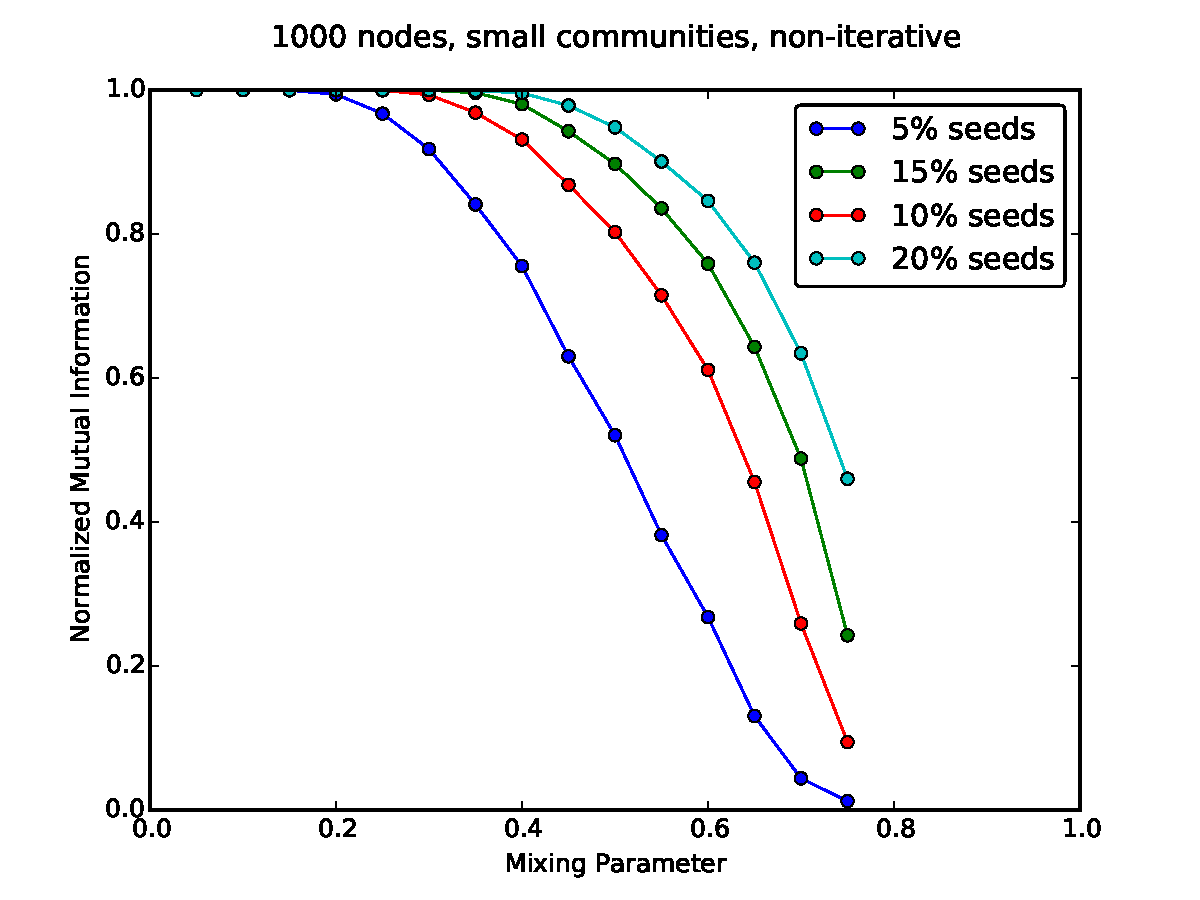
\includegraphics[width=\plotwidth]{plots/nonoverlap_noniter_a.pdf}
    \end{subfigure}%
    \begin{subfigure}{0.5\textwidth}
    \centering
    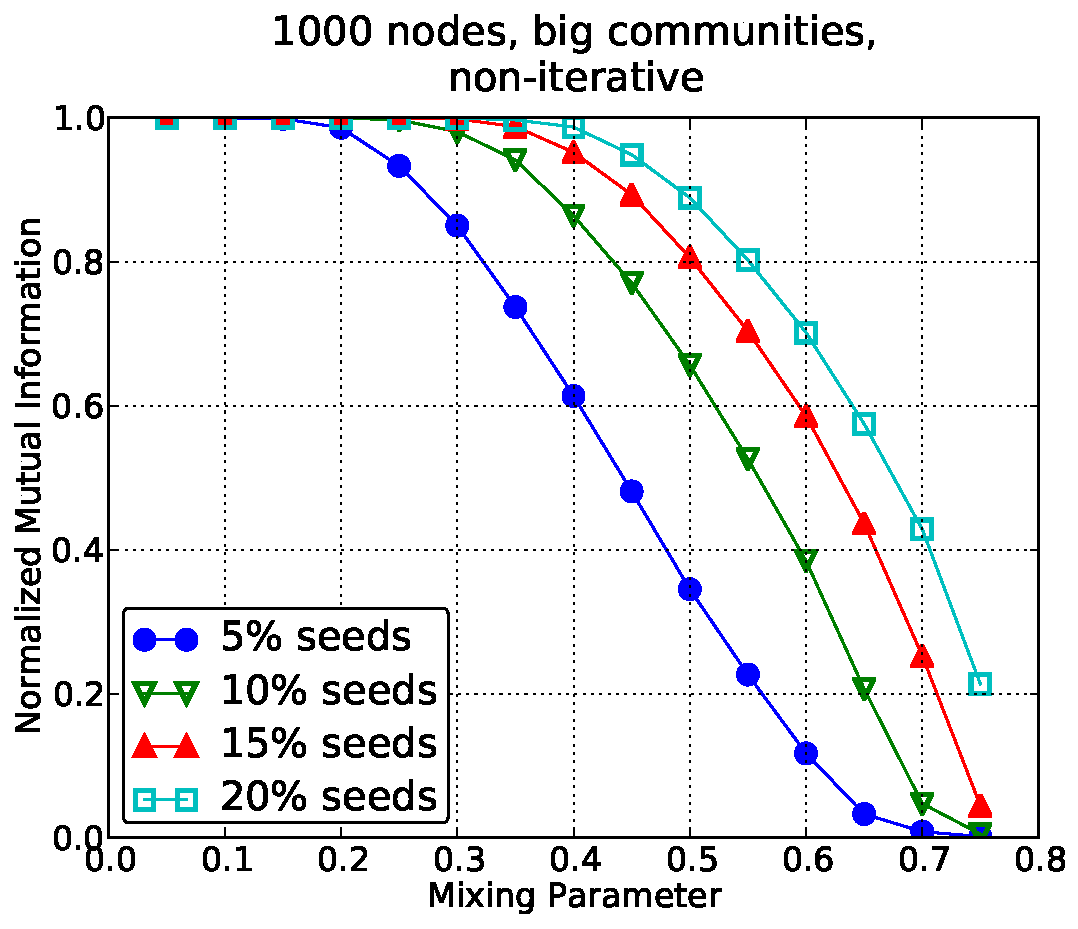
\includegraphics[width=\plotwidth]{plots/nonoverlap_noniter_b.pdf}
    \end{subfigure}
    \begin{subfigure}{0.5\textwidth}
    \centering
    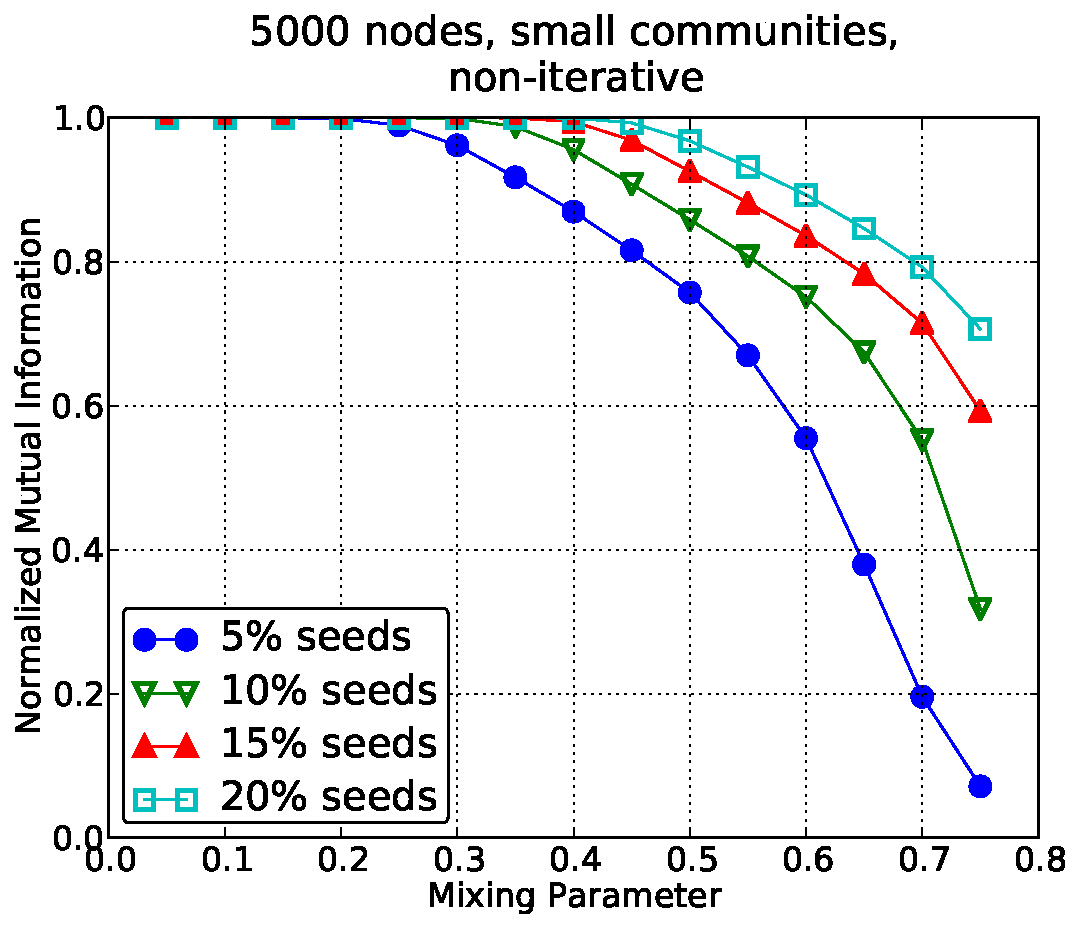
\includegraphics[width=\plotwidth]{plots/nonoverlap_noniter_c.pdf}
    \end{subfigure}%
    \begin{subfigure}{0.5\textwidth}
    \centering
    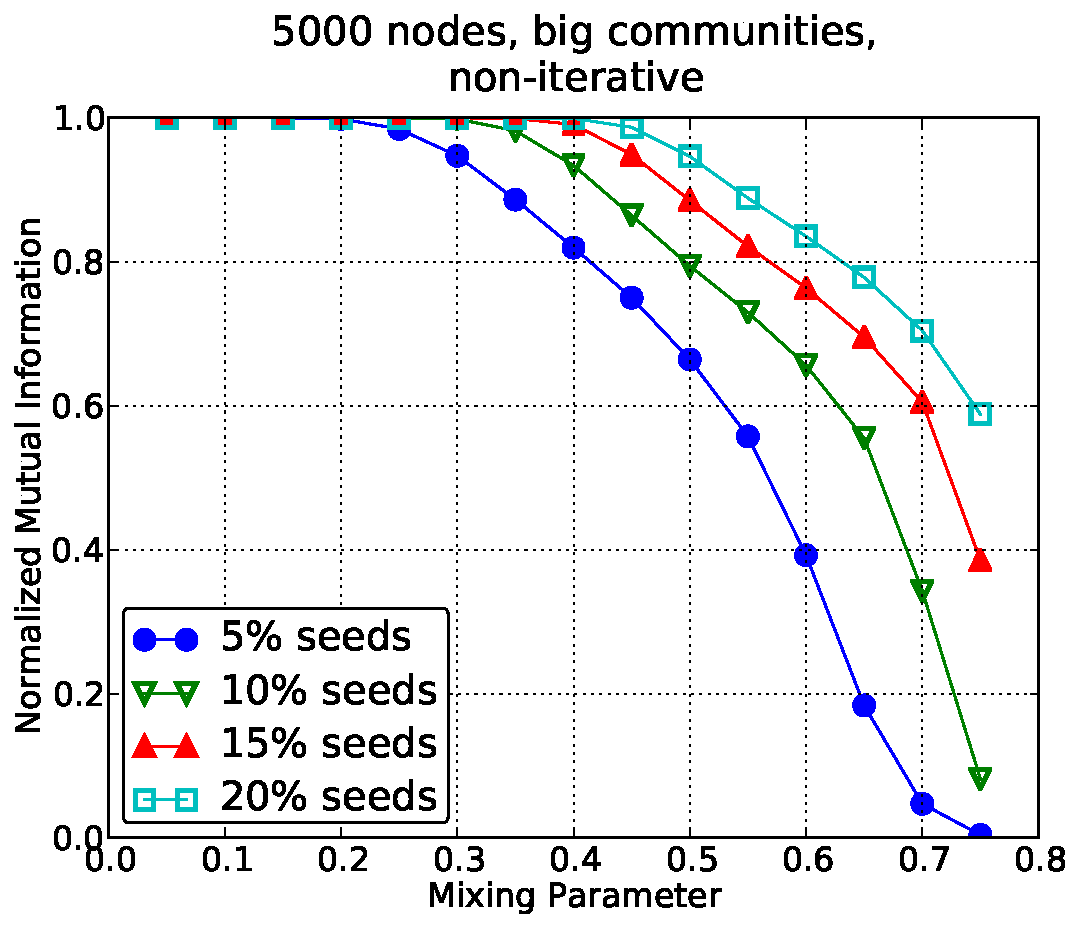
\includegraphics[width=\plotwidth]{plots/nonoverlap_noniter_d.pdf}
    \end{subfigure}
    \caption{Noniterative method for nonoverlapping communities.}\label{fig:no_iter_no_overlap}
\end{figure}

\begin{figure}
    \centering
    \begin{subfigure}{0.5\textwidth}
    \centering
    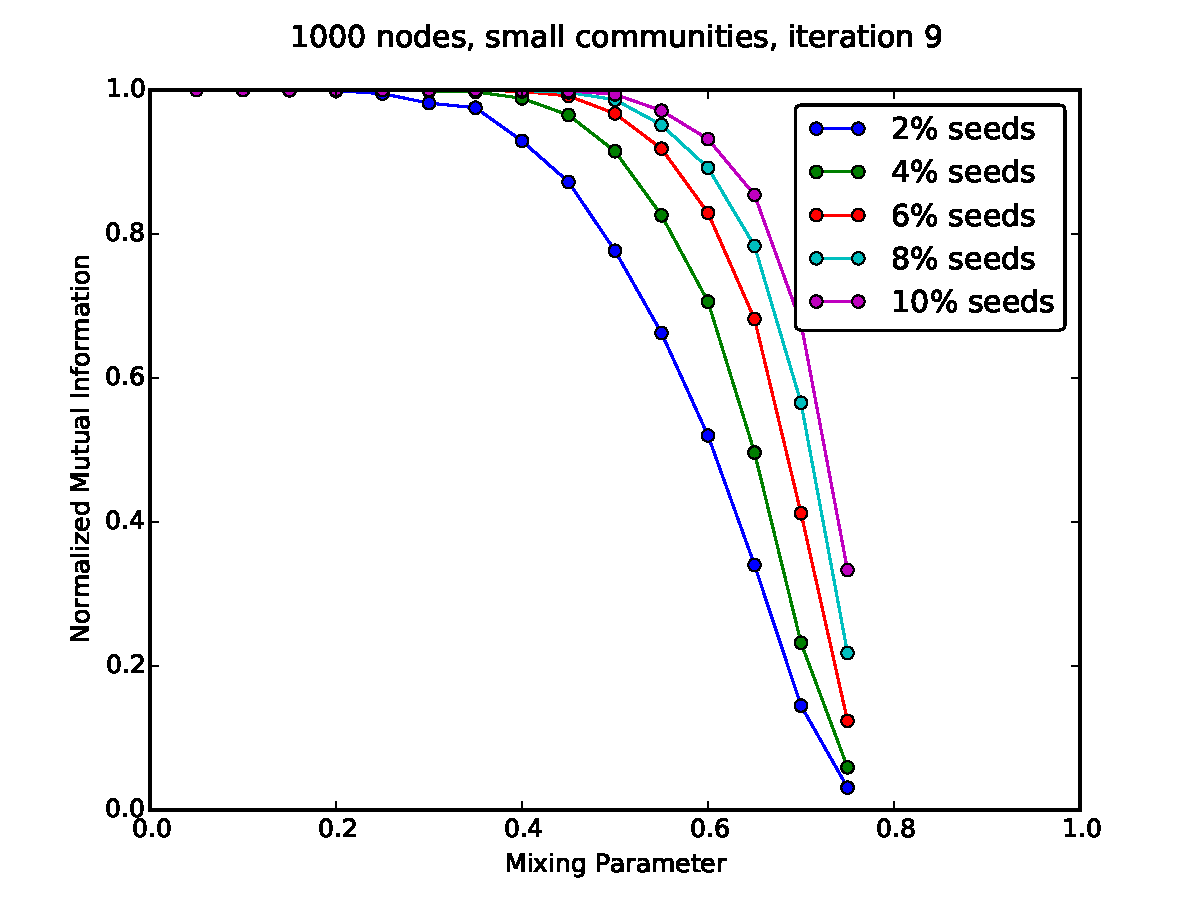
\includegraphics[width=\plotwidth]{plots/nonoverlap_iter_a.pdf}
    \end{subfigure}%
    \begin{subfigure}{0.5\textwidth}
    \centering
    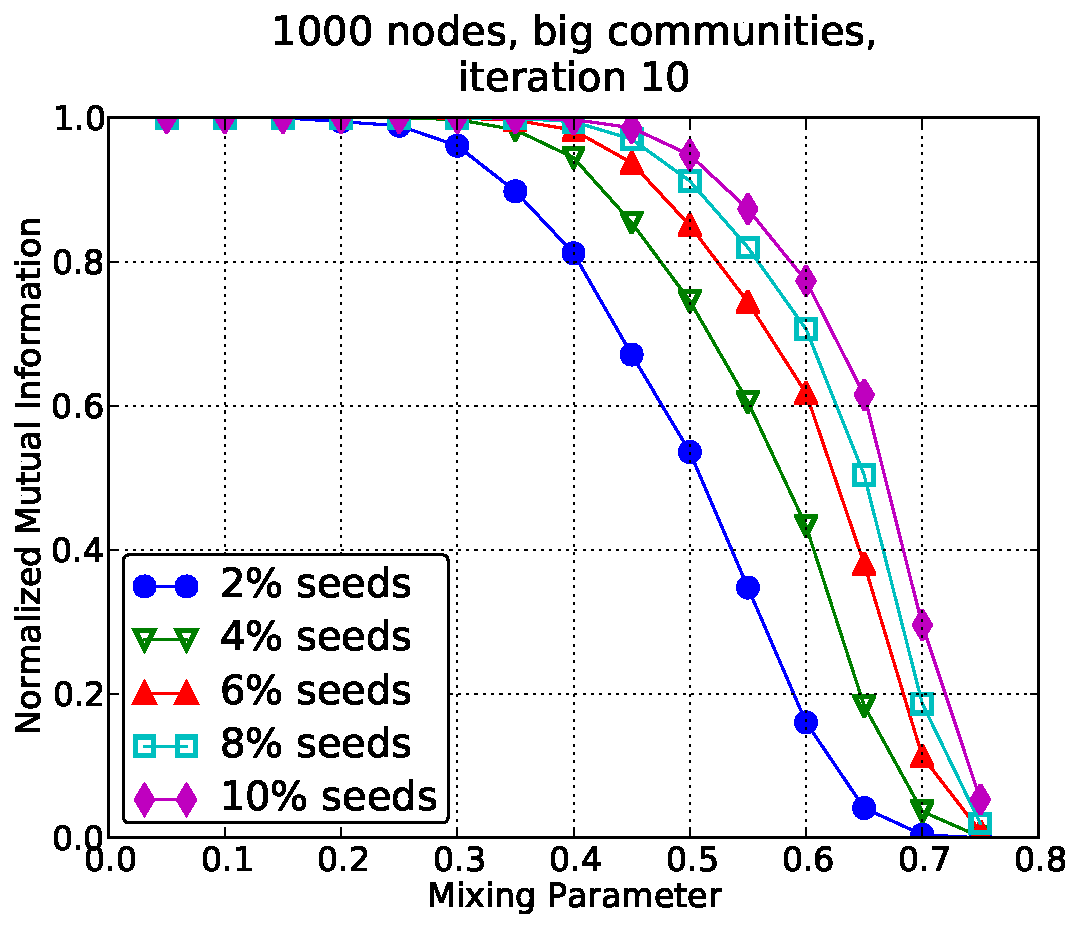
\includegraphics[width=\plotwidth]{plots/nonoverlap_iter_b.pdf}
    \end{subfigure}
    \begin{subfigure}{0.5\textwidth}
    \centering
    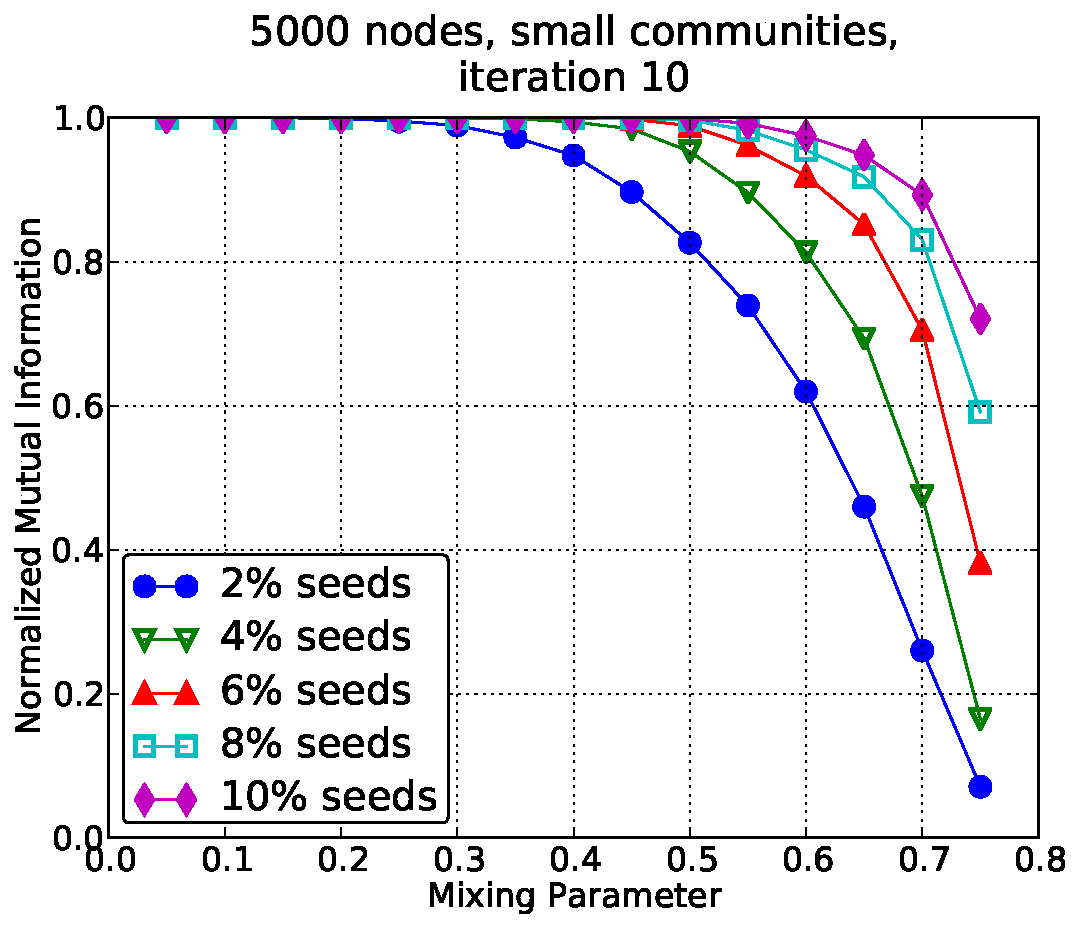
\includegraphics[width=\plotwidth]{plots/nonoverlap_iter_c.pdf}
    \end{subfigure}%
    \begin{subfigure}{0.5\textwidth}
    \centering
    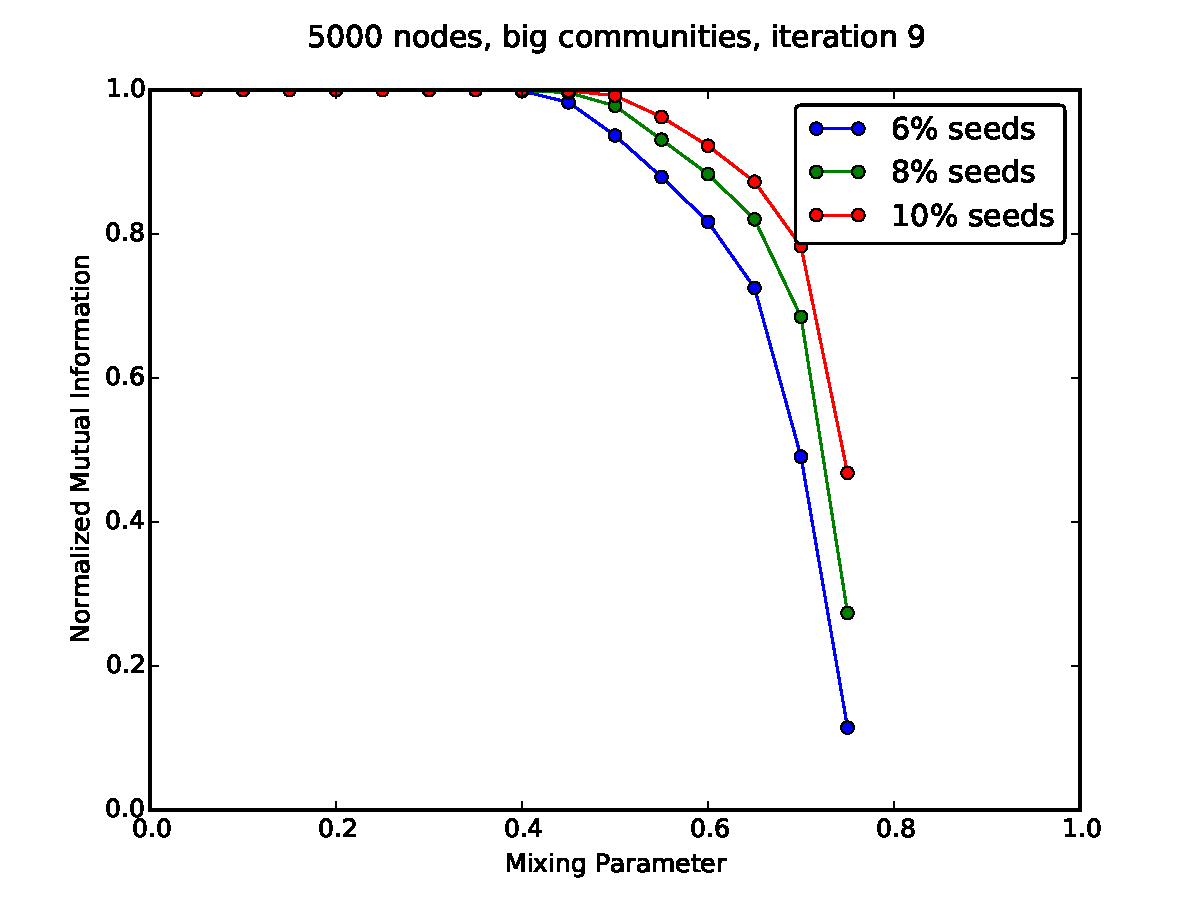
\includegraphics[width=\plotwidth]{plots/nonoverlap_iter_d.pdf}
    \end{subfigure}
    \caption{Iterative method for nonoverlapping communities.}\label{fig:iter_no_overlap}
\end{figure}

\begin{figure}
    \centering
    \begin{subfigure}{0.5\textwidth}
    \centering
    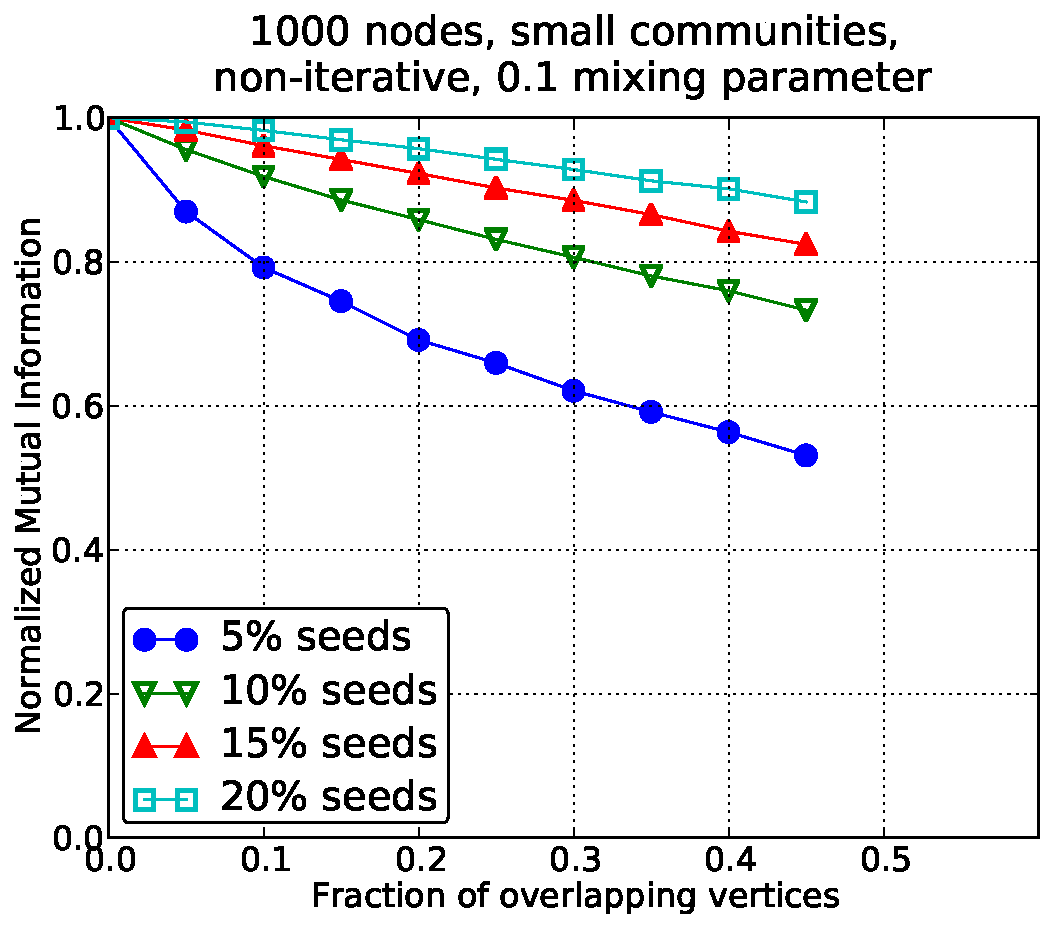
\includegraphics[width=\plotwidth]{plots/overlap_noniter_1mu_a.pdf}
    \end{subfigure}%
    \begin{subfigure}{0.5\textwidth}
    \centering
    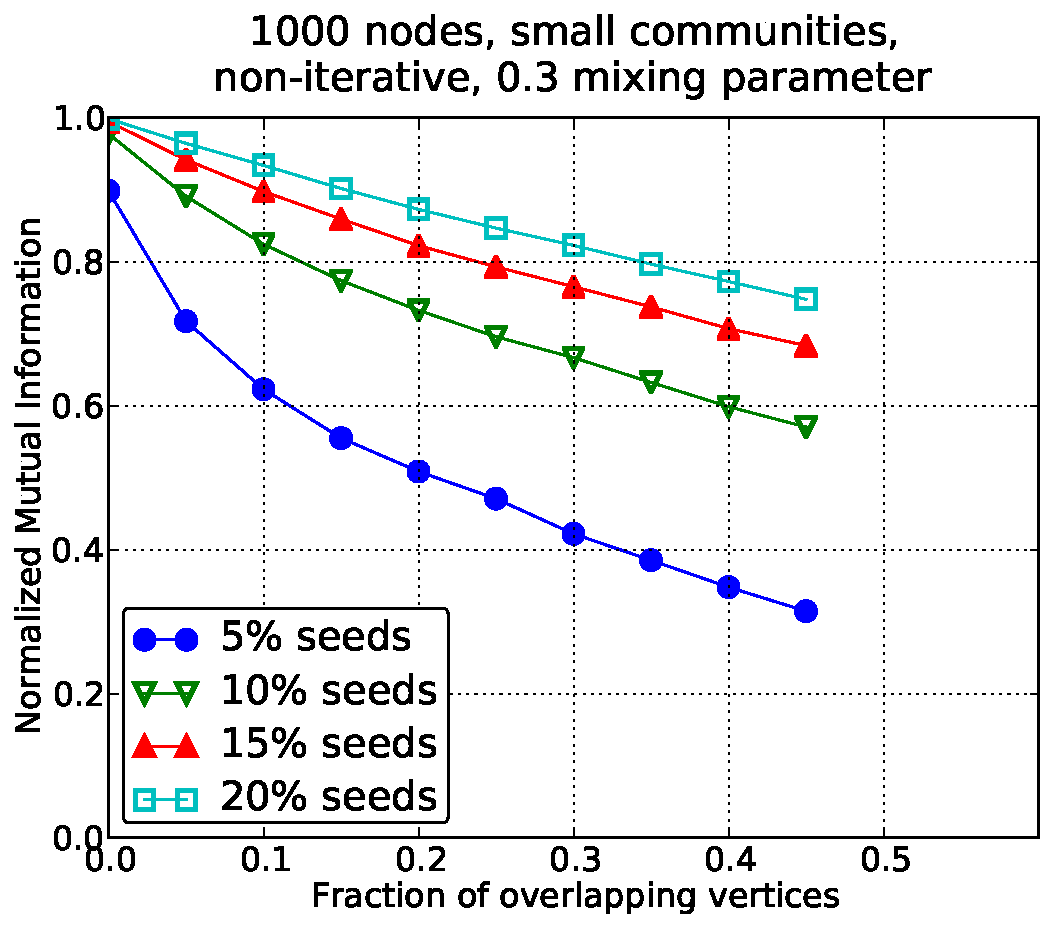
\includegraphics[width=\plotwidth]{plots/overlap_noniter_3mu_a.pdf}
    \end{subfigure}
    \begin{subfigure}{0.5\textwidth}
    \centering
    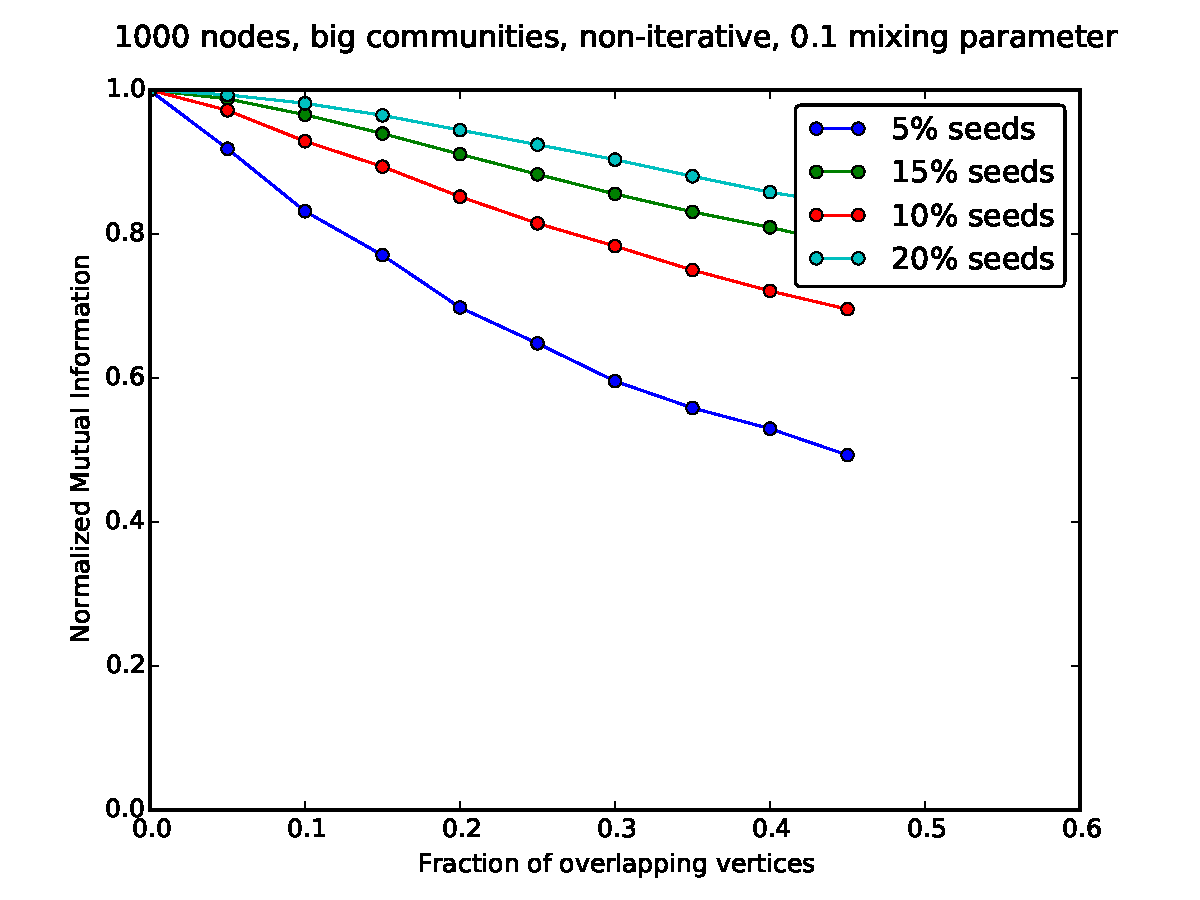
\includegraphics[width=\plotwidth]{plots/overlap_noniter_1mu_b.pdf}
    \end{subfigure}%
    \begin{subfigure}{0.5\textwidth}
    \centering
    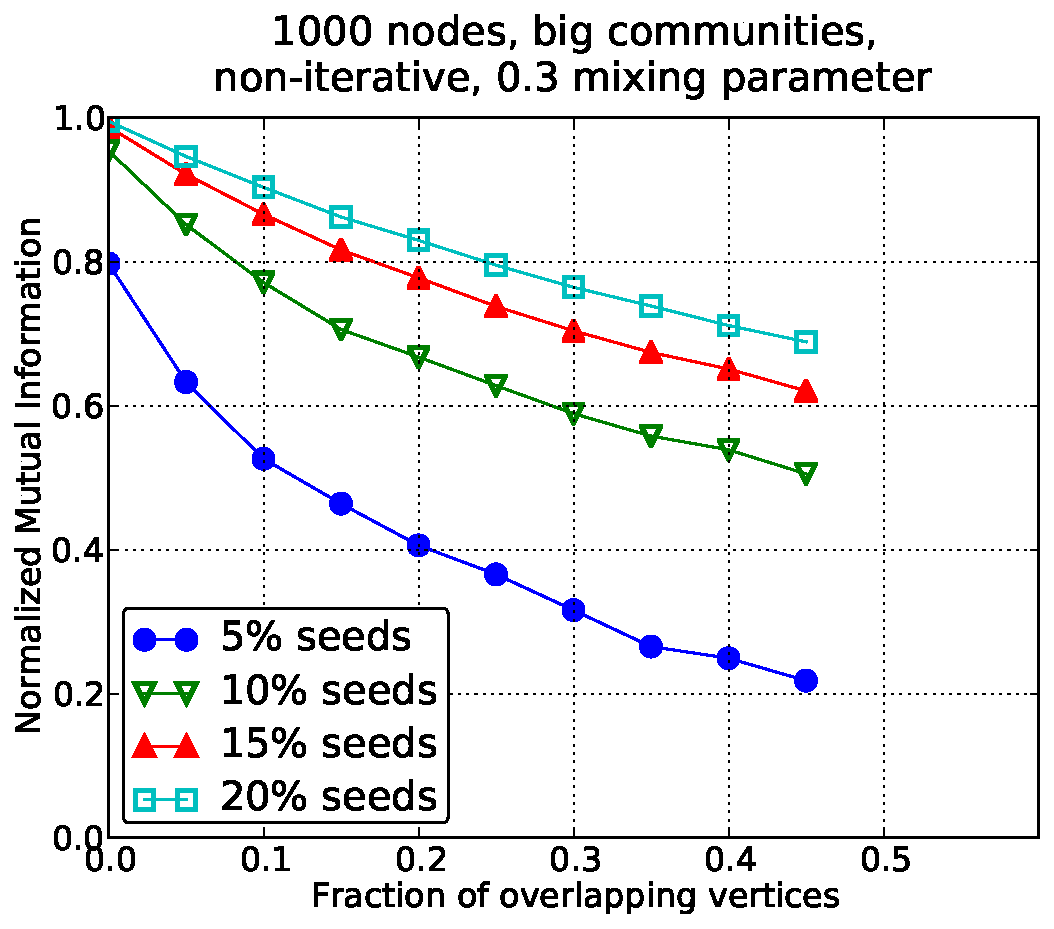
\includegraphics[width=\plotwidth]{plots/overlap_noniter_3mu_b.pdf}
    \end{subfigure}
    \caption{Noniterative method for overlapping communities on 1000 nodes.}\label{fig:no_iter_overlap_1000N}
\end{figure}

\begin{figure}
    \centering
    \begin{subfigure}{0.5\textwidth}
    \centering
    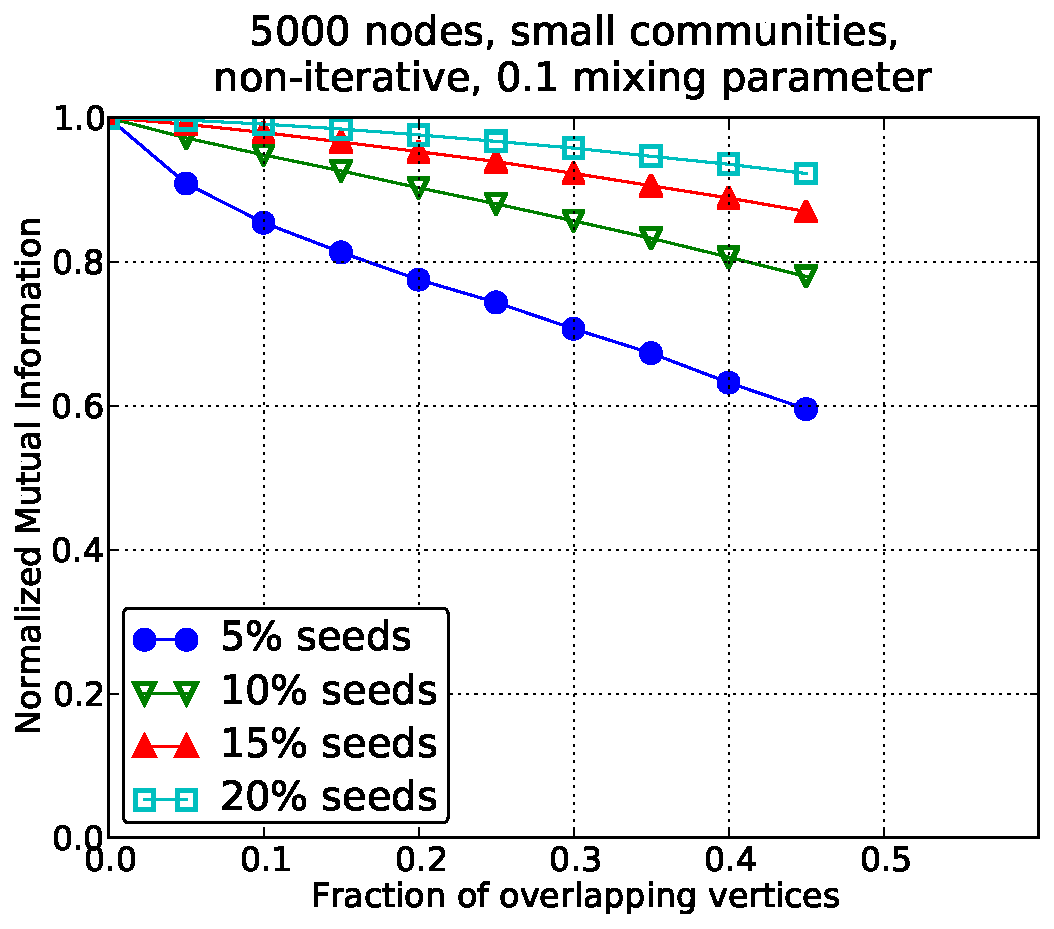
\includegraphics[width=\plotwidth]{plots/overlap_noniter_1mu_c.pdf}
    \end{subfigure}%
    \begin{subfigure}{0.5\textwidth}
    \centering
    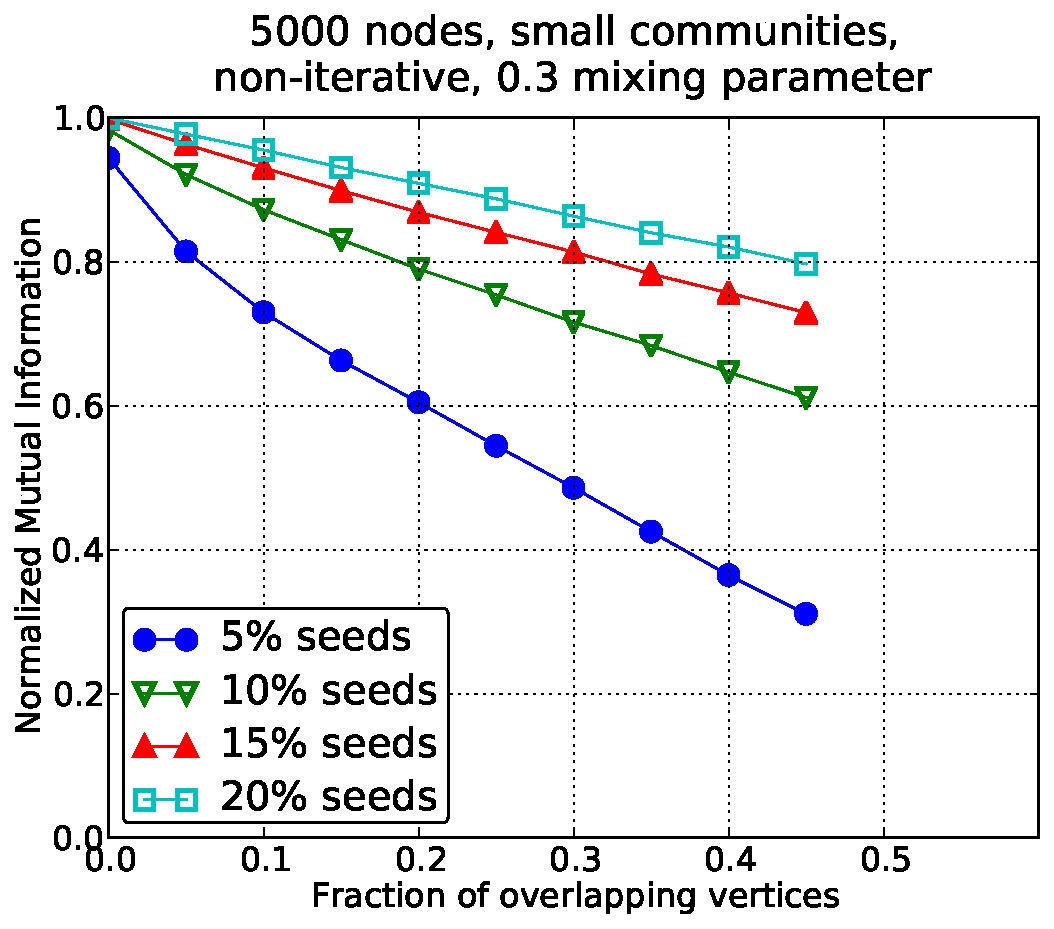
\includegraphics[width=\plotwidth]{plots/overlap_noniter_3mu_c.pdf}
    \end{subfigure}
    \begin{subfigure}{0.5\textwidth}
    \centering
    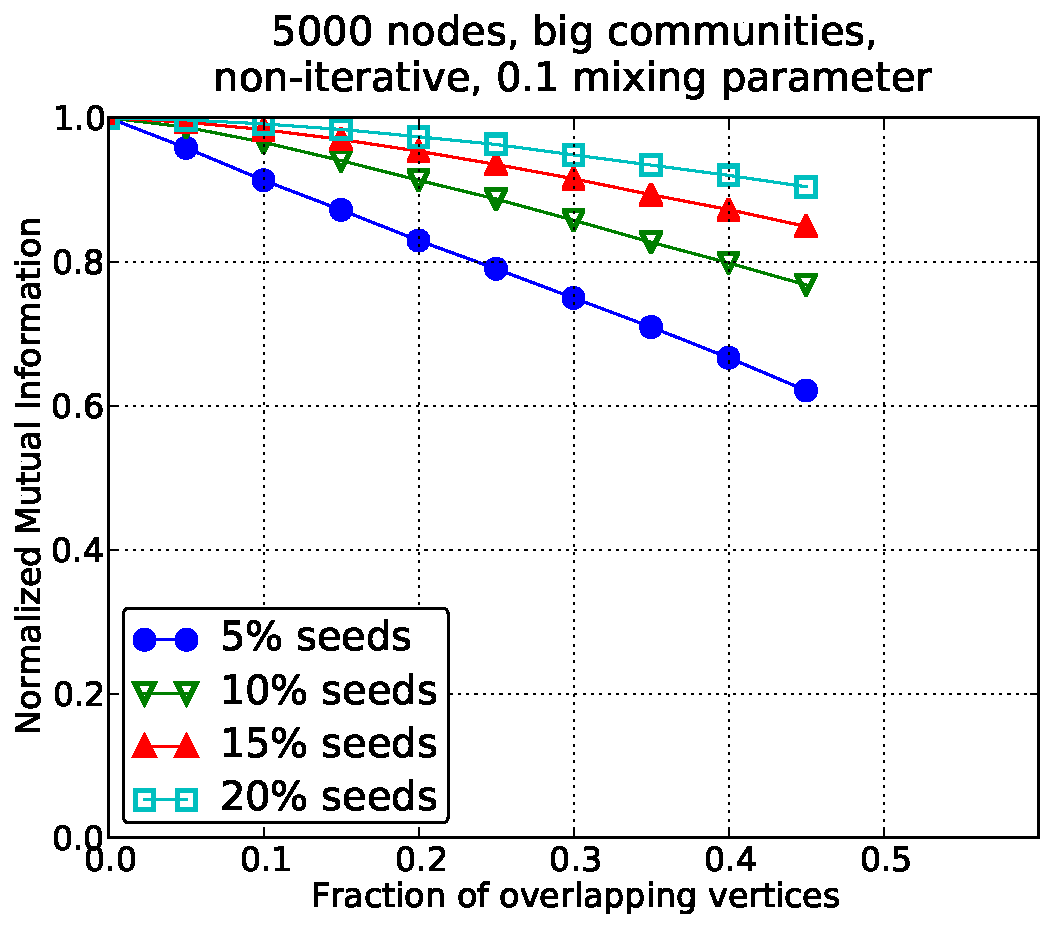
\includegraphics[width=\plotwidth]{plots/overlap_noniter_1mu_d.pdf}
    \end{subfigure}%
    \begin{subfigure}{0.5\textwidth}
    \centering
    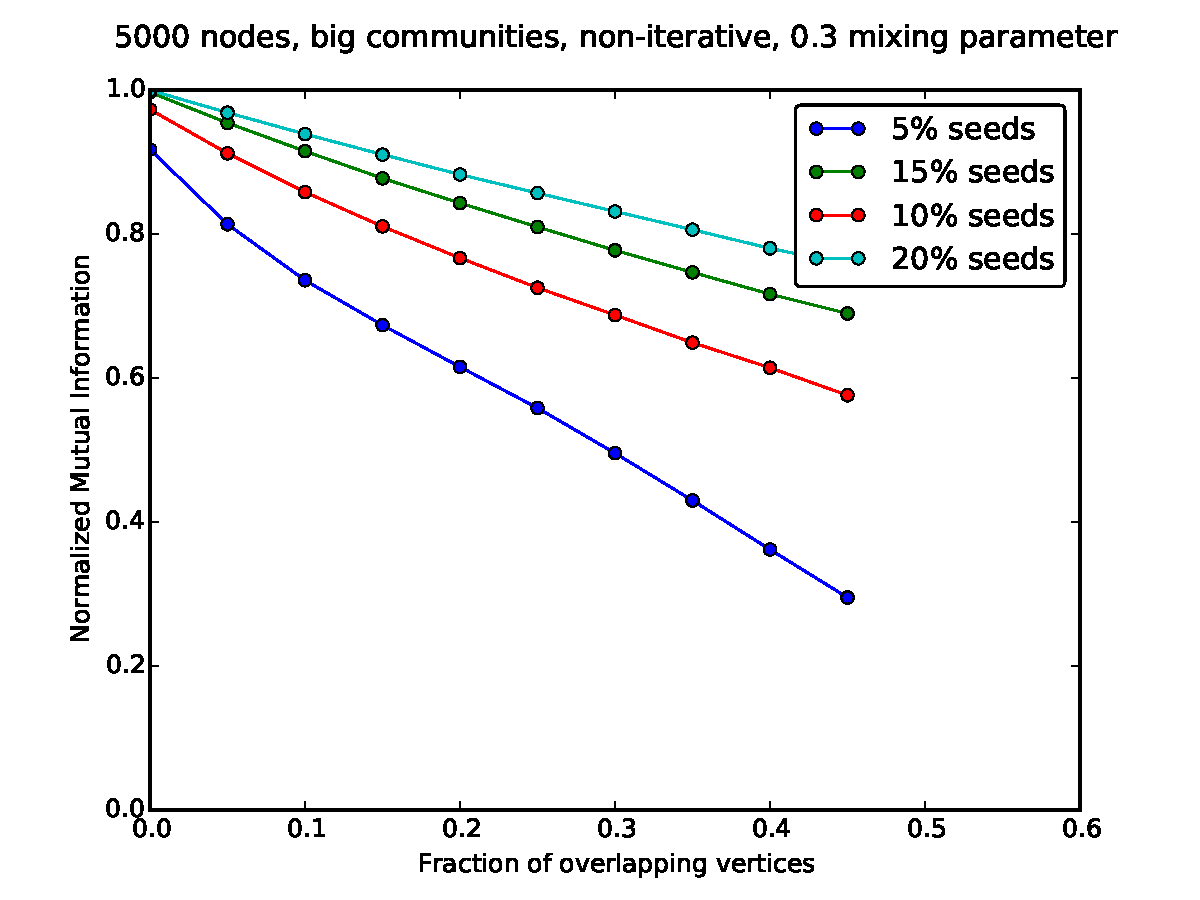
\includegraphics[width=\plotwidth]{plots/overlap_noniter_3mu_d.pdf}
    \end{subfigure}
    \caption{Noniterative method for overlapping communities on 5000 nodes.}\label{fig:no_iter_overlap_5000N}
\end{figure}


\begin{figure}
    \centering
    \begin{subfigure}{0.5\textwidth}
    \centering
    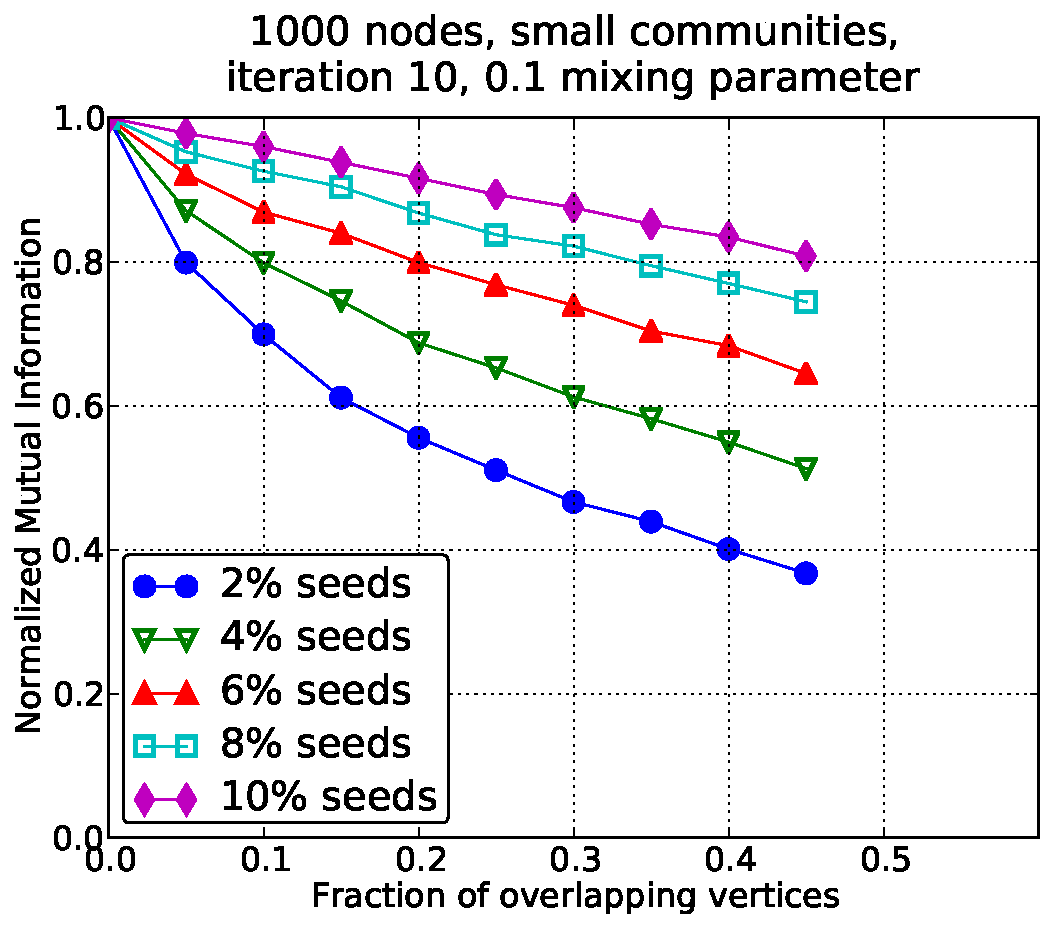
\includegraphics[width=\plotwidth]{plots/overlap_iter_1mu_a.pdf}
    \end{subfigure}%
    \begin{subfigure}{0.5\textwidth}
    \centering
    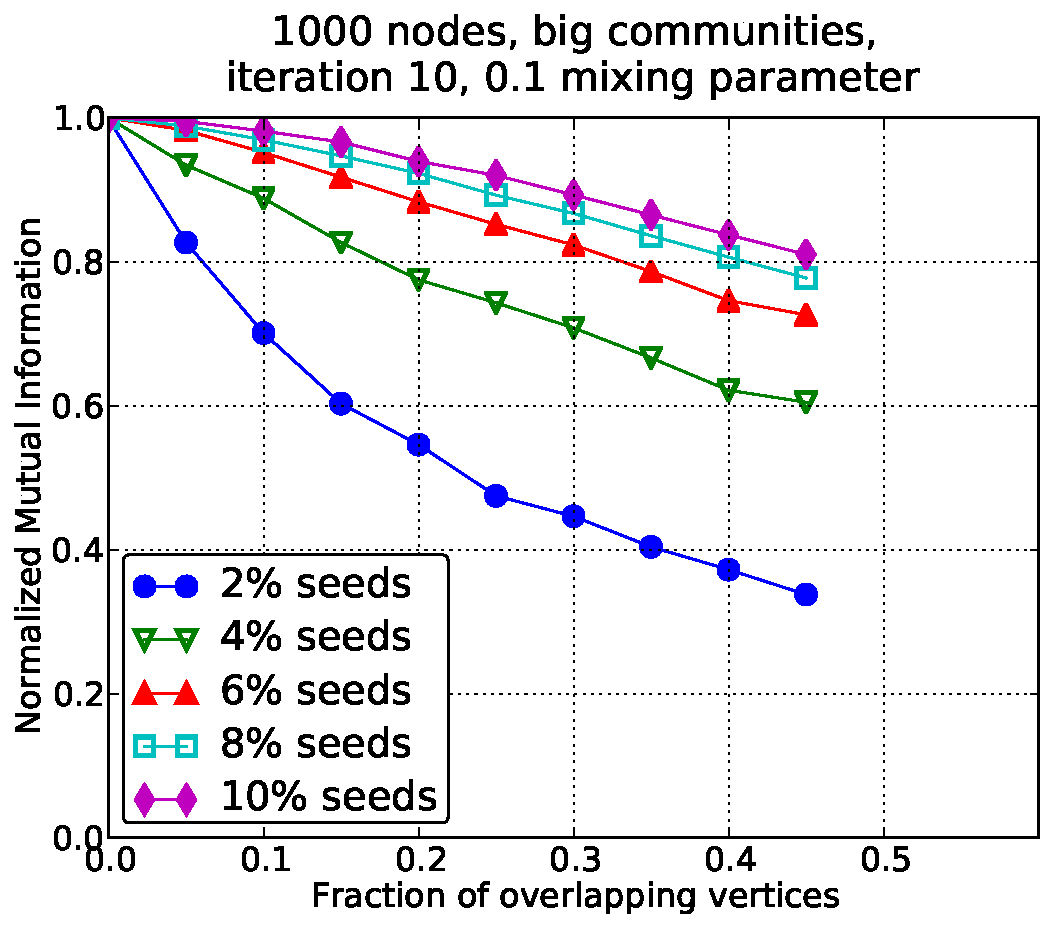
\includegraphics[width=\plotwidth]{plots/overlap_iter_1mu_b.pdf}
    \end{subfigure}
    \begin{subfigure}{0.5\textwidth}
    \centering
    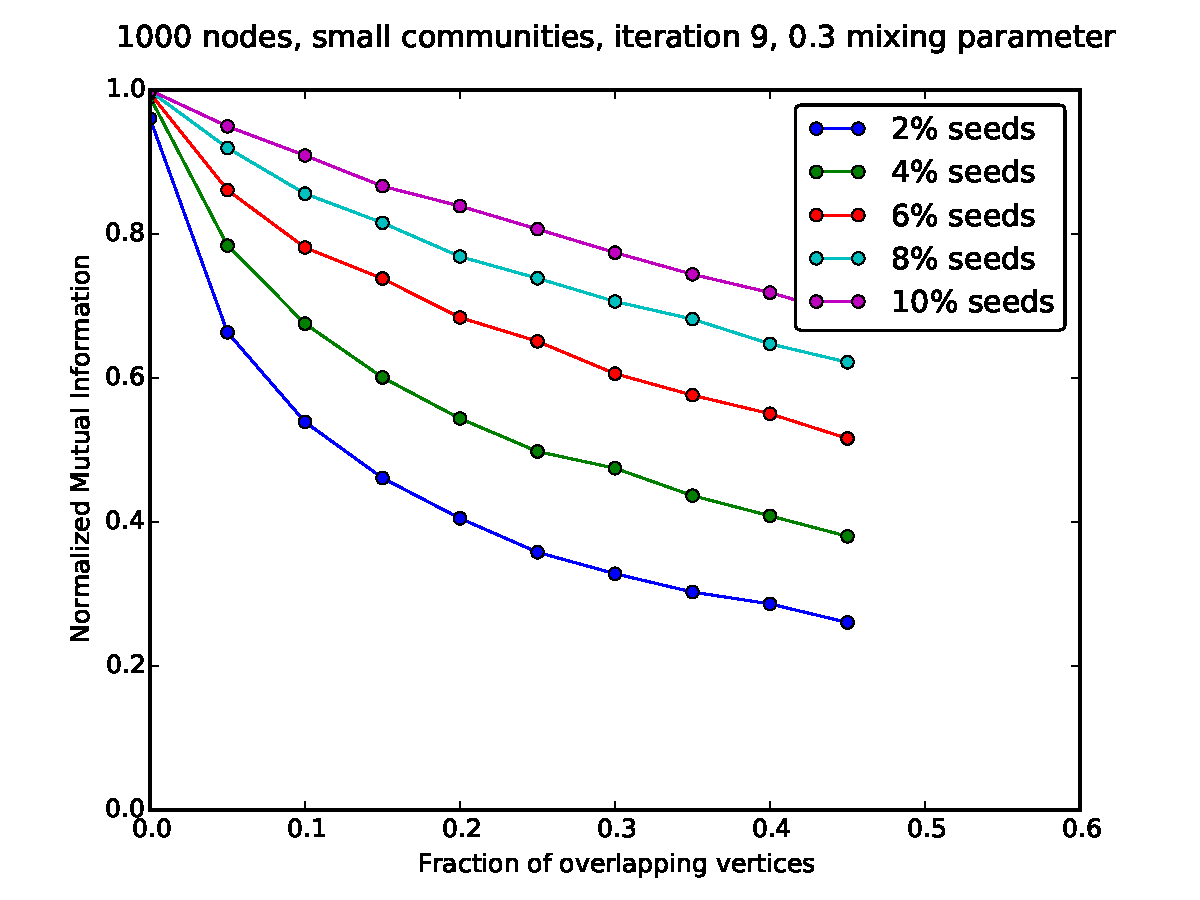
\includegraphics[width=\plotwidth]{plots/overlap_iter_3mu_a.pdf}
    \end{subfigure}%
    \begin{subfigure}{0.5\textwidth}
    \centering
    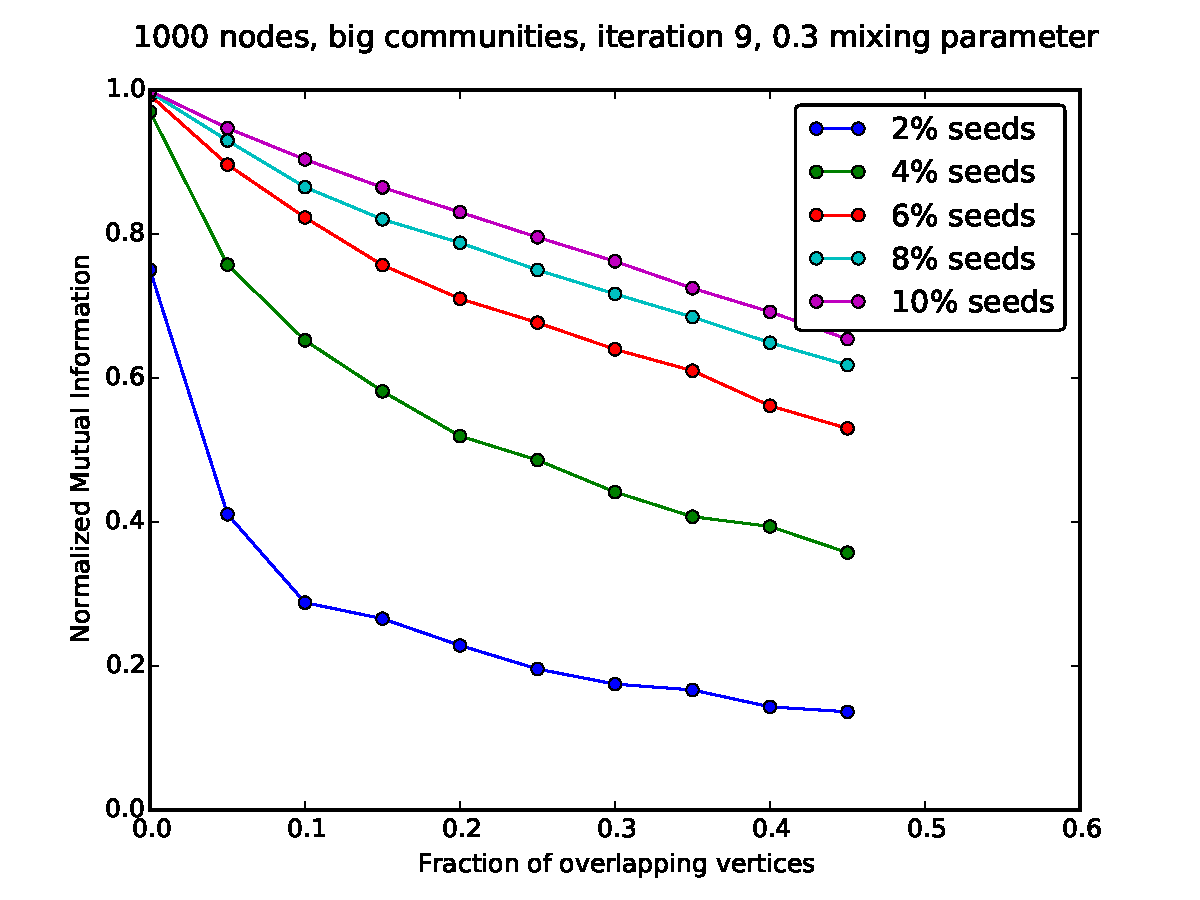
\includegraphics[width=\plotwidth]{plots/overlap_iter_3mu_b.pdf}
    \end{subfigure}
    \caption{Iterative method for overlapping communities on 1000 nodes.}\label{fig:iter_overlap_1000N}
\end{figure}

\begin{figure}
    \centering
    \begin{subfigure}{0.5\textwidth}
    \centering
    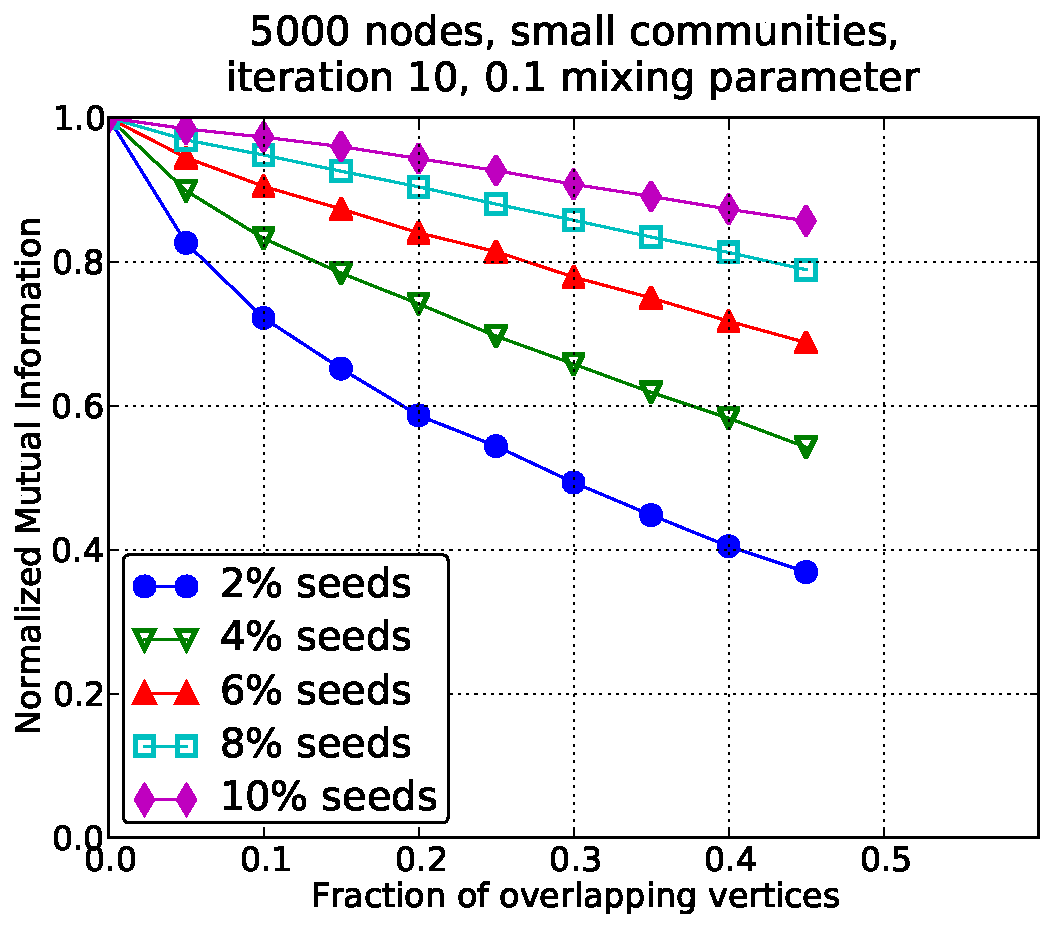
\includegraphics[width=\plotwidth]{plots/overlap_iter_1mu_c.pdf}
    \end{subfigure}%
    \begin{subfigure}{0.5\textwidth}
    \centering
    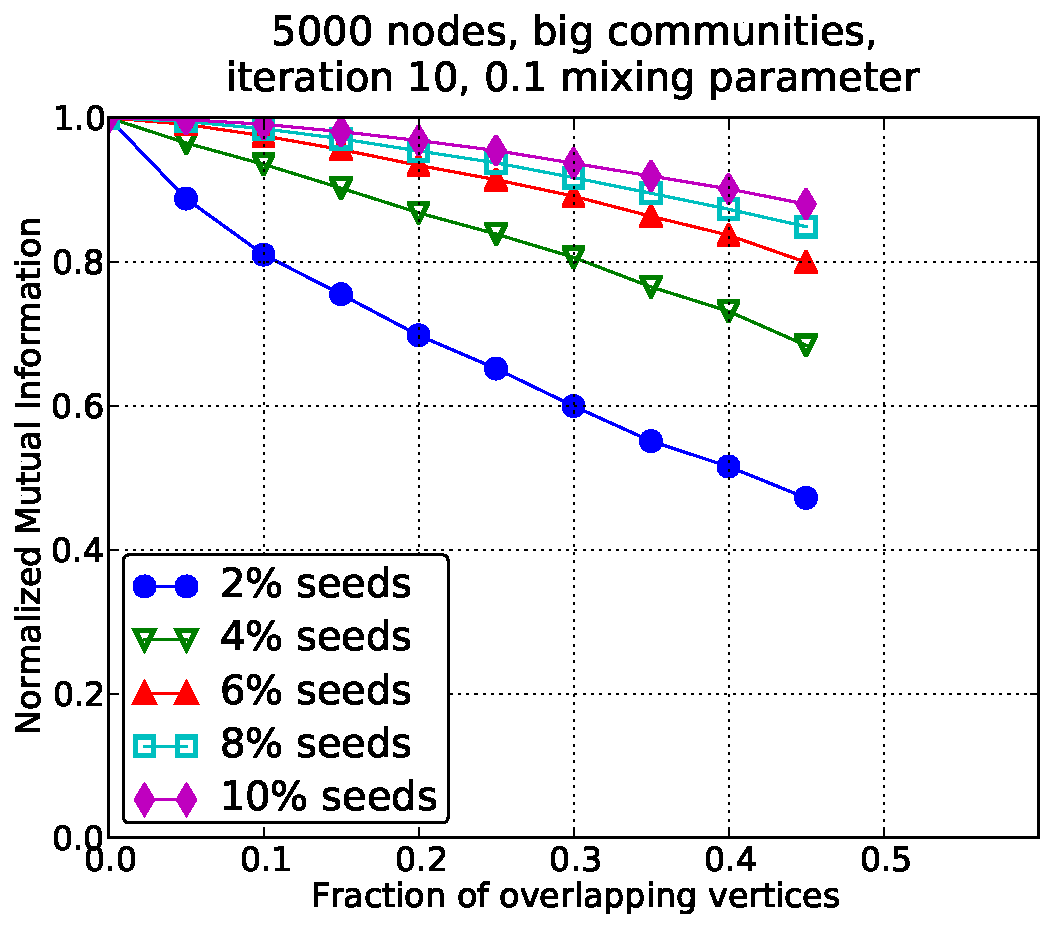
\includegraphics[width=\plotwidth]{plots/overlap_iter_1mu_d.pdf}
    \end{subfigure}
    \begin{subfigure}{0.5\textwidth}
    \centering
    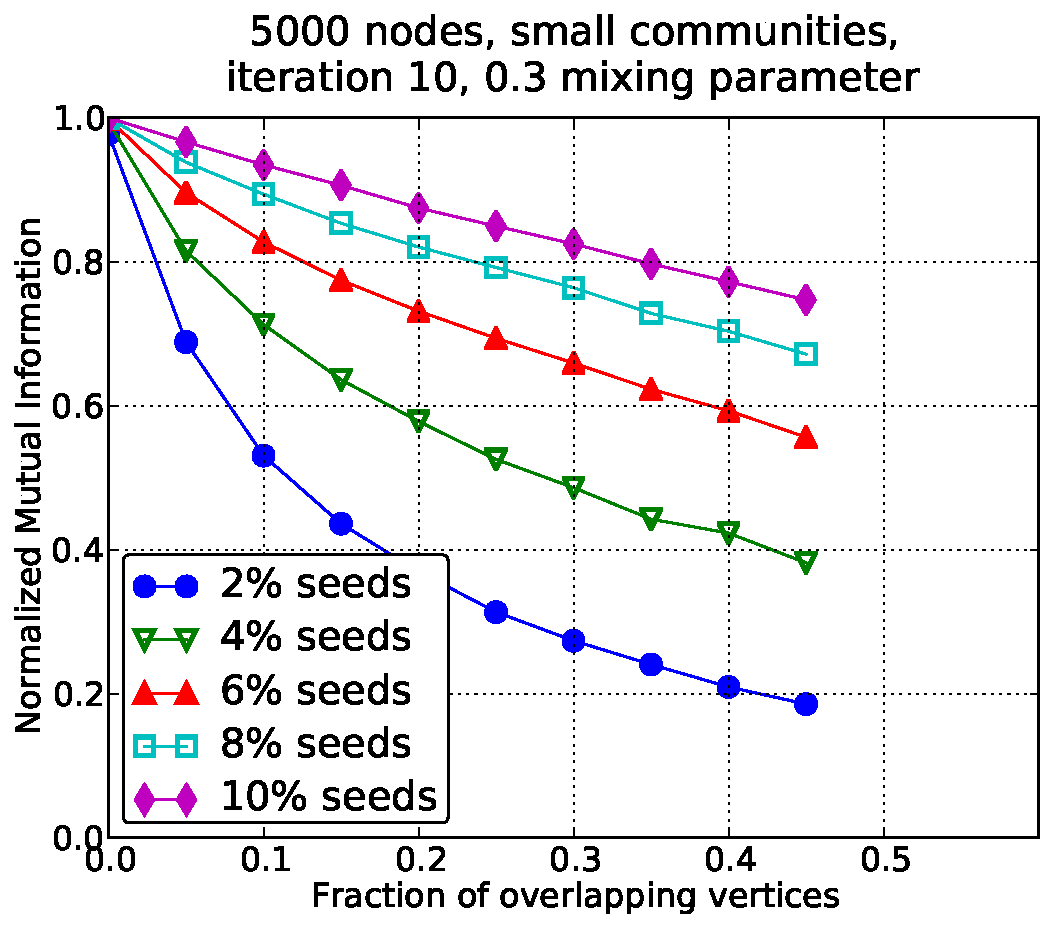
\includegraphics[width=\plotwidth]{plots/overlap_iter_3mu_c.pdf}
    \end{subfigure}%
    \begin{subfigure}{0.5\textwidth}
    \centering
    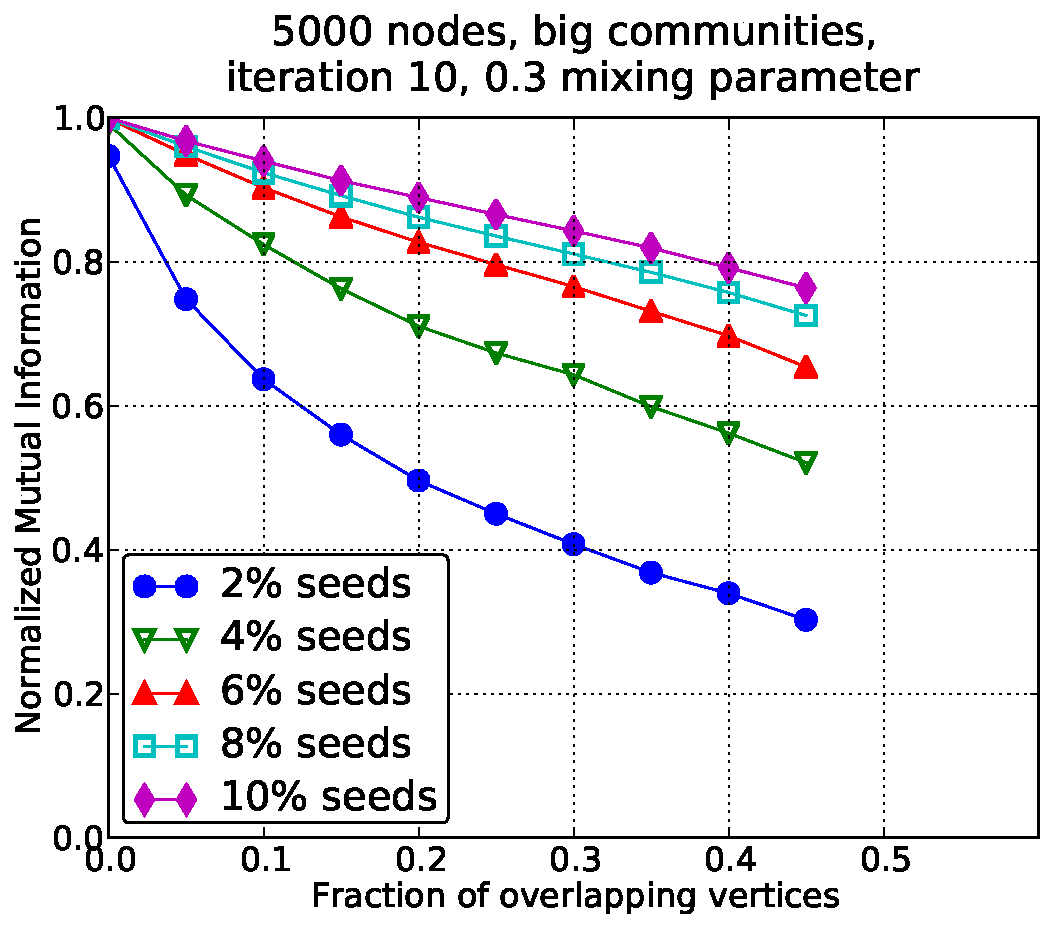
\includegraphics[width=\plotwidth]{plots/overlap_iter_3mu_d.pdf}
    \end{subfigure}
    \caption{Iterative method for overlapping communities on 5000 nodes.}\label{fig:iter_overlap_5000N}
\end{figure}

\begin{figure}
    \centering
    \begin{subfigure}{0.5\textwidth}
    \centering
    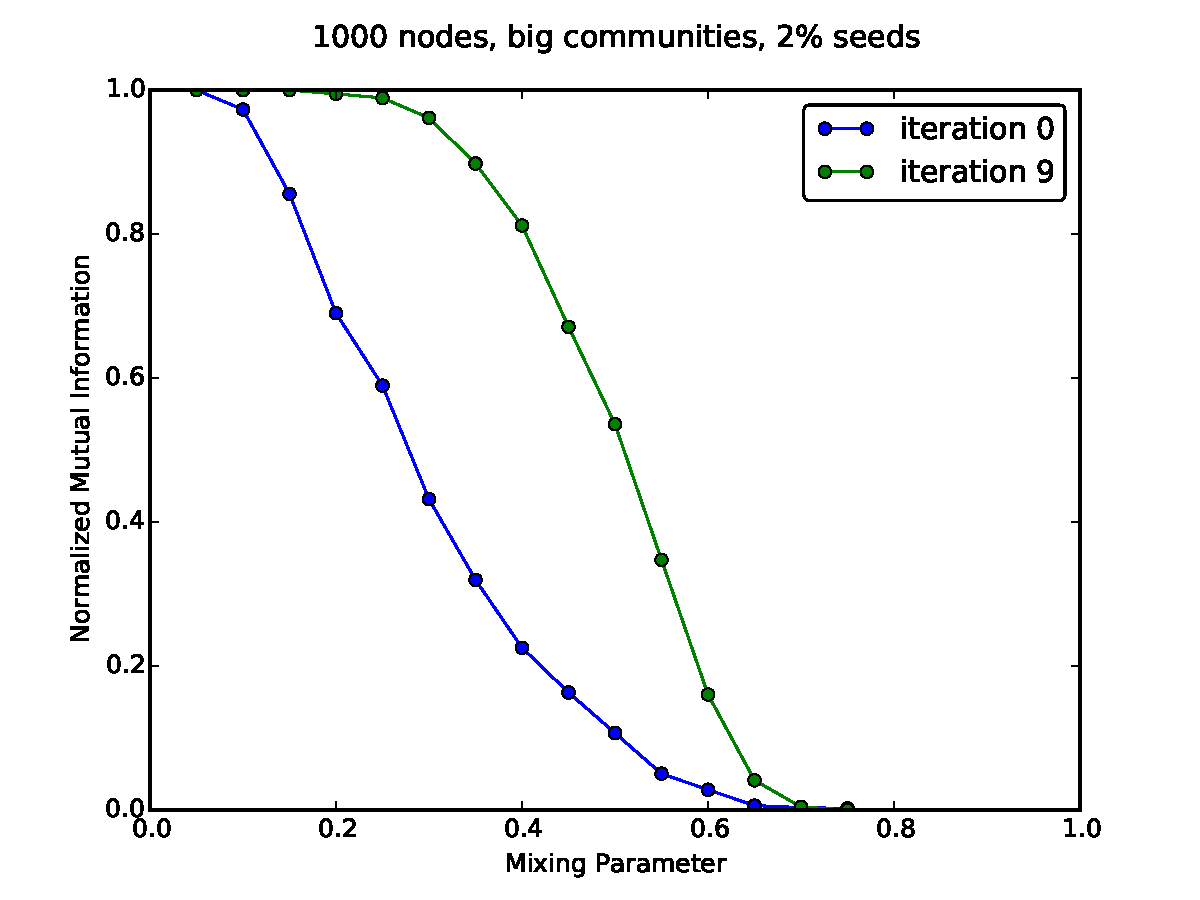
\includegraphics[width=\plotwidth]{plots/nonoverlap_compare_a.pdf}
    \end{subfigure}%
    \begin{subfigure}{0.5\textwidth}
    \centering
    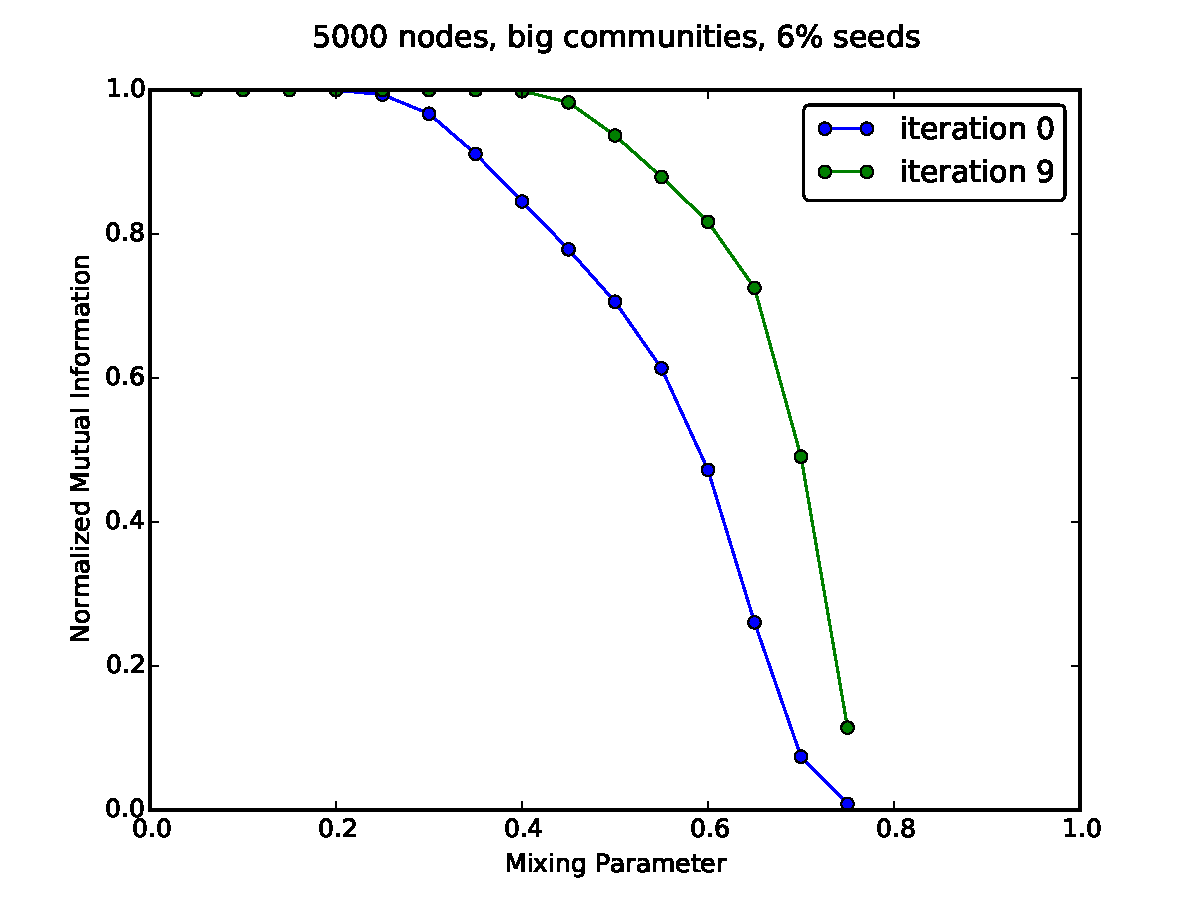
\includegraphics[width=\plotwidth]{plots/nonoverlap_compare_b.pdf}
    \end{subfigure}
    \caption{Comparison between the the iterative and non-iterative method for non-overlapping communities.}\label{fig:compare_iter_no_overlap}
\end{figure}


\begin{figure}
    \centering
    \begin{subfigure}{0.5\textwidth}
    \centering
    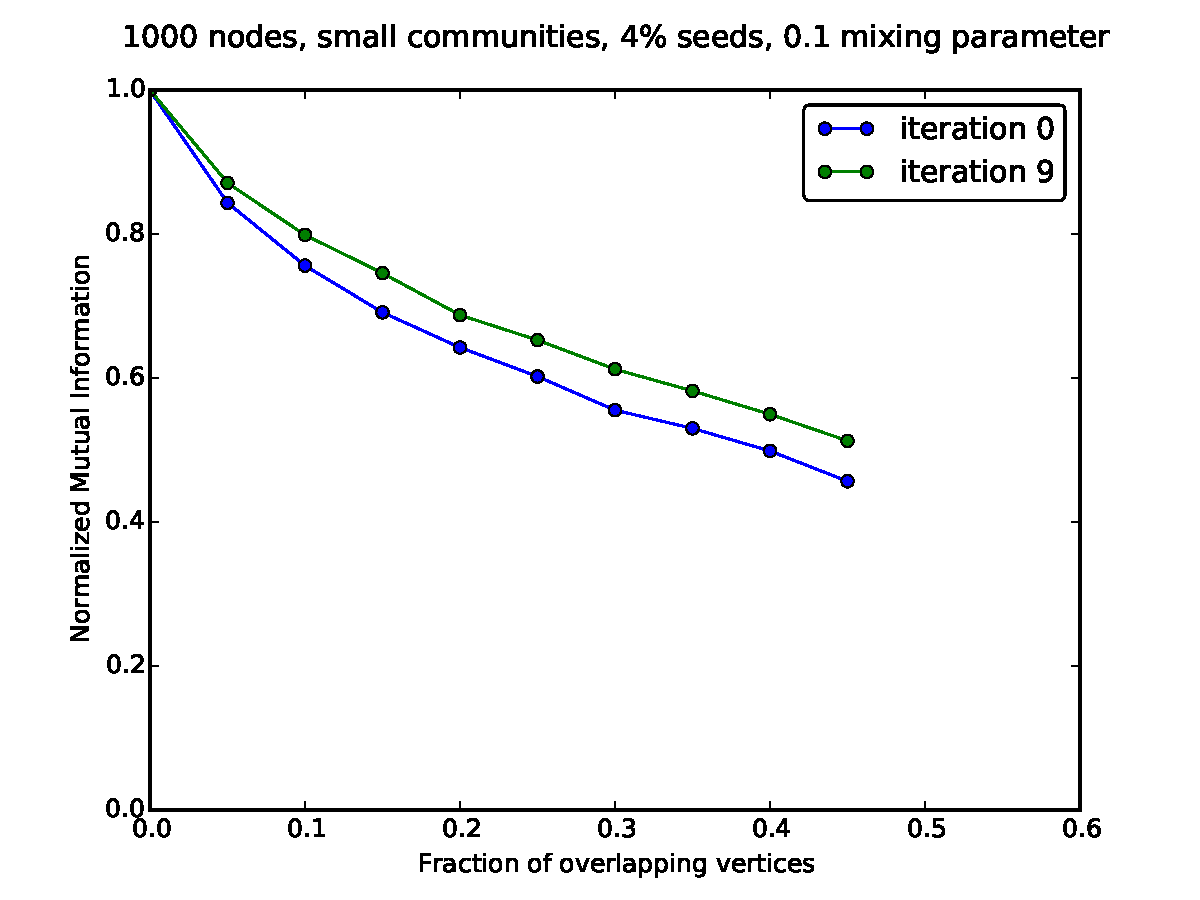
\includegraphics[width=\plotwidth]{plots/overlap_compare_a.pdf}
    \end{subfigure}%
    \begin{subfigure}{0.5\textwidth}
    \centering
    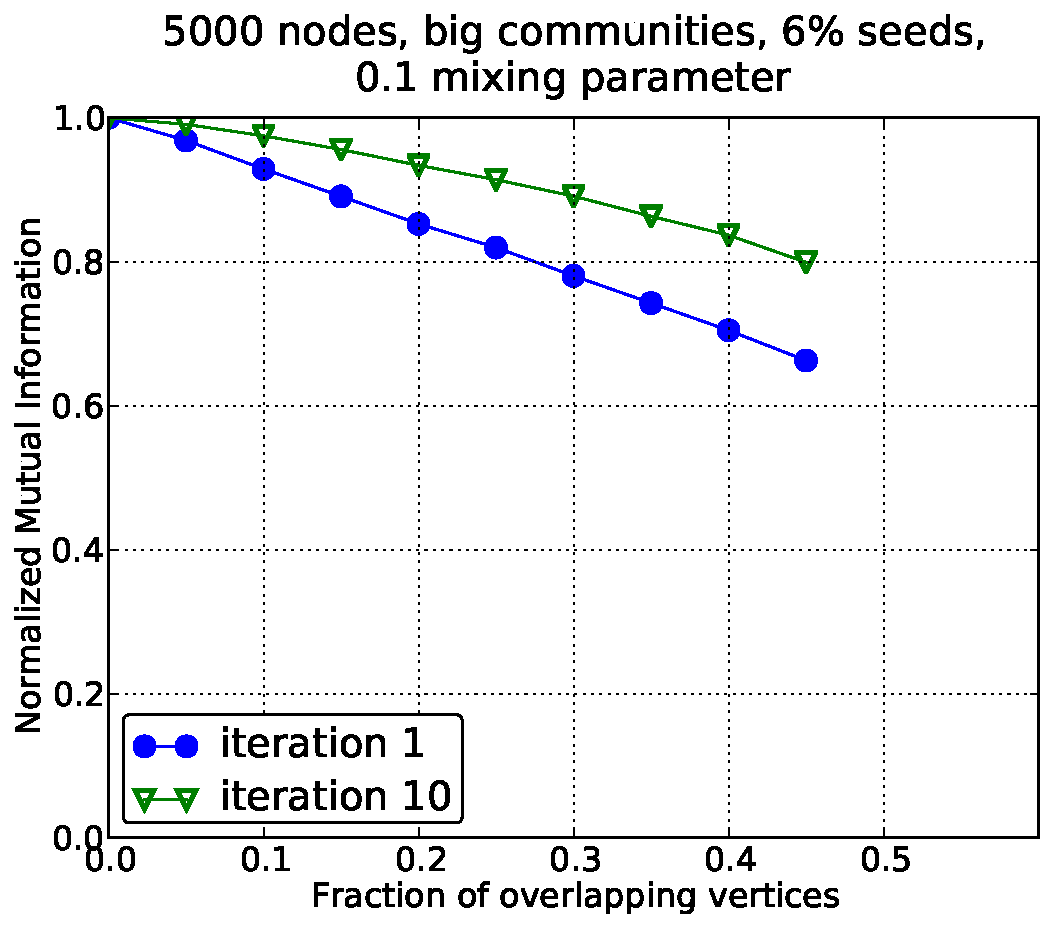
\includegraphics[width=\plotwidth]{plots/overlap_compare_b.pdf}
    \end{subfigure}
    \caption{Comparison between the the iterative and non-iterative method for overlapping communities.}\label{fig:compare_iter_overlap}
\end{figure}


\begin{figure}
    \centering
    \texttt{TODO: add plots}
    %\includegraphics{}
    \caption{
        Test of Infomap, CFinder, Clauset et al, Girvan Newman (GN) and Blonel et al on the LFR benchmark for the nonoverlapping communities. 
        Tests were performed on graphs with 1000 and 5000 nodes with big (B) and small (S) communities.
        These figures are taken from \texttt{name of the paper}.
    }
\end{figure}


\newcommand{\cfinderwidth}{0.96\linewidth}
\begin{figure}
    \centering
    \begin{subfigure}{0.5\textwidth}
    \centering
    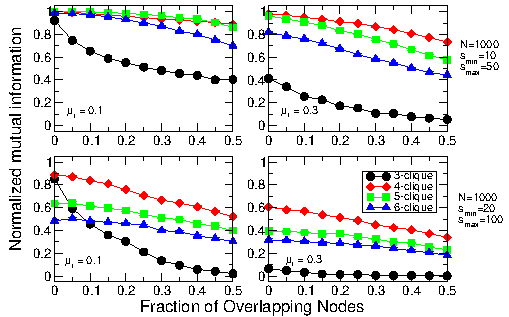
\includegraphics[width=\cfinderwidth]{lfrpaper/fig6.pdf}
    \end{subfigure}%
    \begin{subfigure}{0.5\textwidth}
    \centering
    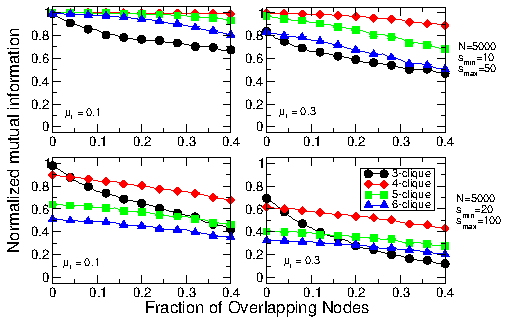
\includegraphics[width=\cfinderwidth]{lfrpaper/fig7.pdf}
    \end{subfigure}%
    \caption{
        Test of CFinder on the LFR benchmark with overlapping communities.
        Tests were performed on graphs with 1000 and 5000 nodes.
        These figures are taken from \texttt{name of the paper}.
    }
\end{figure}



%\begin{figure}
    %\centering
    %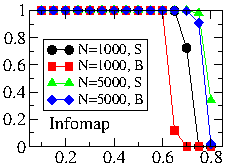
\includegraphics{lfrpaper/fig2_b.pdf}
%\end{figure}

%\begin{figure}
    %\centering
    %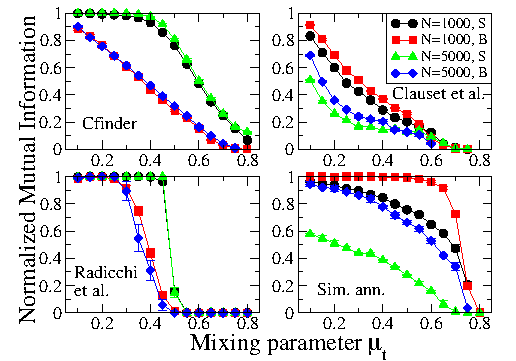
\includegraphics{lfrpaper/fig2_b_sub.pdf}
%\end{figure}

%\begin{figure}
    %\centering
    %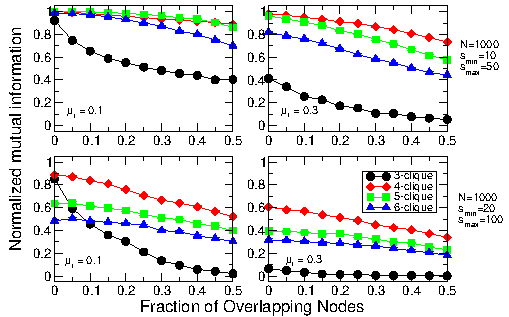
\includegraphics{lfrpaper/fig6.pdf}
%\end{figure}

%\begin{figure}
    %\centering
    %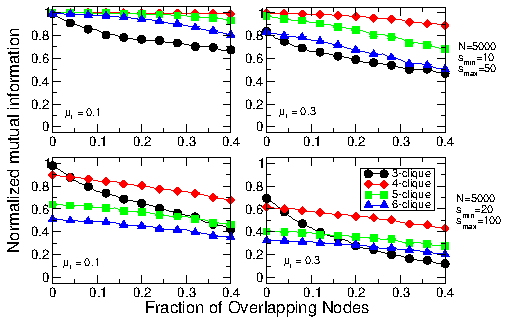
\includegraphics{lfrpaper/fig7.pdf}
%\end{figure}

